% Synopsis "Fælles aner" — forblad, synopsis og bilag i ét dokument.
% Kompileres med: pdflatex synopsis.tex   (MiKTeX, dansk tegnsæt via inputenc/T1)
% Kodeuddragene er hentet fra src/ på dev-branchen (okt. 2026); koden er uden
% kommentarer og docstrings, så forklaringerne står i teksten. Figurene
% genereres af synopsis/figurer/make_figures.py.
\documentclass[12pt, a4paper]{article}
\usepackage[utf8]{inputenc}
\usepackage[T1]{fontenc}
\usepackage{lmodern}
\usepackage{geometry}
\geometry{margin=2.5cm}
\usepackage{amsmath, amssymb}
\usepackage{graphicx}
\usepackage{booktabs}
\usepackage{listings}
\usepackage{xcolor}
\usepackage{caption}
\usepackage[colorlinks=true, linkcolor=blue, urlcolor=blue]{hyperref}

\lstset{
    basicstyle=\ttfamily\small,
    keywordstyle=\color{blue},
    commentstyle=\color{gray},
    stringstyle=\color{teal},
    numbers=left,
    numberstyle=\tiny\color{gray},
    breaklines=true,
    frame=single,
    tabsize=4,
    showstringspaces=false,
    literate={æ}{{\ae}}1 {ø}{{\o}}1 {å}{{\aa}}1
             {Æ}{{\AE}}1 {Ø}{{\O}}1 {Å}{{\AA}}1
             {§}{{\S}}1 {—}{{---}}1 {–}{{--}}1
             {Θ}{{$\Theta$}}1 {α}{{$\alpha$}}1 {φ}{{$\varphi$}}1
             {≤}{{$\leq$}}1 {→}{{$\rightarrow$}}1 {∪}{{$\cup$}}1
             {Ē}{{$\bar{E}$}}1 {⁻}{{$^-$}}1 {̃}{{\~{}}}1
}

\title{Synopsis --- \textit{Fælles aner}}
\author{[projektdeltagere]}
\date{}
\emergencystretch=2em

\begin{document}

% ─────────────────────────────────────────────────────────────────────────────
% FORBLAD
% ─────────────────────────────────────────────────────────────────────────────
\thispagestyle{empty}
\begin{center}
{\LARGE\bfseries Fælles aner}\\[1em]
{\large Programmeringsprojekt --- synopsis}\\[2.5em]
\begin{tabular}{ll}
Projektdeltagere: & \textit{(navne indsættes her)} \\
Klasse: & 3.O \\
Dato: & \textit{(afleveringsdato indsættes her)} \\
\end{tabular}
\end{center}

\vspace{3em}
\noindent Synopsis til projektet \emph{Fælles aner} (afsnit 7.10). Det fulde
program ligger i repoet
\url{https://github.com/ExperiencesXP/proj_herritage_tree} på branchen
\texttt{dev}. Bilagene efter synopsen dokumenterer koden, figurene,
udviklingsprocessen og kravopfyldelsen.

\newpage

% ─────────────────────────────────────────────────────────────────────────────
\section*{1. Projektbeskrivelse}
% ─────────────────────────────────────────────────────────────────────────────

Programmet \emph{Fælles aner} undersøger slægtskab i en familie og besvarer
spørgsmålet fra afsnit 7.10: \emph{har to personer mindst en fælles ane?}
Familien modelleres som en graf, hvor hver person er en knude, og hver
forældreference (\texttt{mom}/\texttt{dad}) er en rettet kant fra forælder til
barn. Da en person højst har to forældre, er antallet af kanter $m \le 2n$
(invariant \textbf{I1}).

To idéer bærer projektet. For det første opdeles befolkningen i \emph{klynger}:
de sammenhængende komponenter af den udretningsløse skygge $\bar{E}$, hvor
kanternes retning ignoreres --- alle slægtninge i en familie hænger sammen,
mens personer fra forskellige familier ikke gør. For det andet beregnes
forfædre-mængden $\mathrm{Anc}(v)$ rekursivt som det mindste faste punkt for
operatoren $\Phi_v(S)$ (\S 2.5 i designdokumentet), og to personer er
beslægtede netop når deres to mængder skærer hinanden.

Matematikken er dokumenteret i designdokumentet
(\path{docs/cluster_map_and_recursive_search.md}, 528 linjer med beviser):
klusterkortet kan bygges i $\Theta(n)$ tid og plads, fordi $m \le 2n$
(\S 4.1); antallet af klynger $k$ og vellykkede sammenlægninger $s$ opfylder
identitet (3) $k = n - s$ (teorem 3.3); og pedigree-collapse (invariant
\textbf{I3}) viser, at antallet af forfædre er langt mindre end den naive
binære grænse, når familier gentagne ganger blander slægtninge --- målt
$|\mathrm{Anc}(v_k)| = 3k + 1$ for diamantkæden $D_k$ mod grænsen
$2^{2k+1} - 1$ (figur i bilag C).

% ─────────────────────────────────────────────────────────────────────────────
\section*{2. Funktionsbeskrivelse}
% ─────────────────────────────────────────────────────────────────────────────

Brugeren installerer med \texttt{poetry install} og kører hele programmet med
ét kommando, \texttt{poetry run python src}. Programmet indlæser en befolkning
af personer, bygger klusterkortet og svarer på spørgsmål om familien:
hvilket kluster en person hører til, hvem personens forfædre og efterkommere
er, en målrettet søgning med tidligt stop, og --- som det centrale ---
\texttt{find\_common\_ancestor()} og \texttt{is\_related()}, der besvarer
spørgsmålet om fælles aner. Hvert kluster tegnes som et lagdelt stamtræ med
\texttt{matplotlib.pyplot} og skrives til \texttt{out/}, og hvert kluster kan
desuden eksporteres som Mermaid- eller Graphviz-kode.

Eksempel på udskrift:

\begin{lstlisting}[basicstyle=\ttfamily\footnotesize]
common ancestors of mia and dan: ada
is_related(mia, dan) = True
is_related(kid, solo) = False
\end{lstlisting}

\begin{figure}[h]
\centering
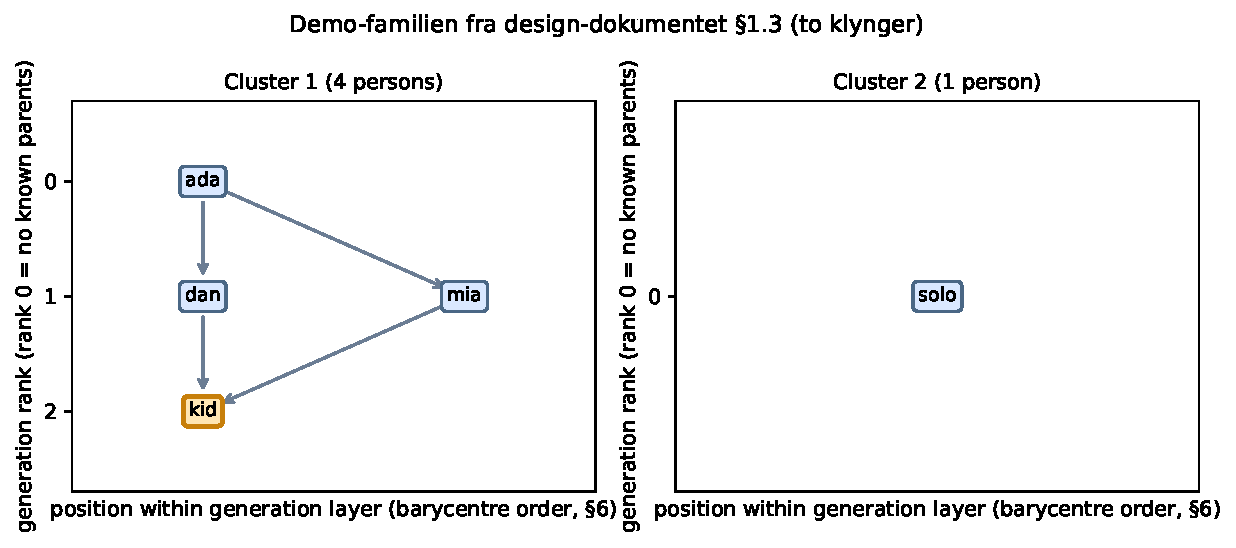
\includegraphics[width=0.85\textwidth]{figurer/familie_demo.pdf}
\caption{Demo-familien tegnet af programmets eget view-modul: to klynger ---
sammenbrudsfamilien til venstre og den isolerede person \texttt{solo} til højre.}
\end{figure}

Den indbyggede demo-familie har to klynger (figuren): en sammenbrudt familie,
hvor \texttt{ada} er forælder til både \texttt{mia} og \texttt{dan}, og den
isolererede person \texttt{solo}. Opgavens \emph{store familie} --- fjorten
personer over fire generationer --- er tegnet færdigt i bilag C, hvor
programmets eget spørgsmål finder de fælles aner for to kusiner.

% ─────────────────────────────────────────────────────────────────────────────
\section*{3. Dokumentation af programmet}
% ─────────────────────────────────────────────────────────────────────────────

Overordnet følger programmet MVC-arkitekturen, som opgaven kræver (bilag A).
\emph{Modellen} er pakken \texttt{src/model/} med data og algoritmer og kender
hverken til visning eller styring; \emph{view}-laget (\texttt{draw.py},
\texttt{view.py}) omsætter resultater til tekstuddrag og matplotlib-figurer;
og \emph{controlleren} (\texttt{controller.py}, \texttt{\_\_main\_\_.py}) ejer
tilstanden og kæder lagene sammen. Pipelinen er: indlæs befolkning $\to$ byg
indeks $\to$ klusterkort $\to$ søgning $\to$ layout $\to$ eksport.

Programmets kerne er klasserne \texttt{Person} og \texttt{Pronouns} (datamodel),
\texttt{FamilyGraph} (grafen), \texttt{Cluster}, \texttt{ClusterMap} og
\texttt{UnionFind} (klusterkortet), \texttt{Layout} (tegningen) og
\texttt{FamilyController} (styringen). Tabellen viser, hvor hver del er
forklaret i detaljer:

\begin{center}\footnotesize
\begin{tabular}{@{}p{3,4cm}p{4,4cm}p{5,8cm}@{}}
\toprule
\textbf{Modul} & \textbf{Klasser} & \textbf{Nøglefunktioner} \\
\midrule
\texttt{model.person} & \texttt{Person}, \texttt{Pronouns} &
  \texttt{\_\_str\_\_}, \texttt{pronoun}, \texttt{from\_preset} (B1) \\
\texttt{model.graph\_model} & \texttt{FamilyGraph} &
  \texttt{build\_family\_graph}, \texttt{parent\_edges} (B2) \\
\texttt{model.search} & \texttt{CycleError} &
  \texttt{explore}, \texttt{ancestors\_iterative},
  \texttt{find\_common\_ancestor}, \texttt{is\_related} (B3, B5, B8) \\
\texttt{model.cluster\_map} & \texttt{Cluster}, \texttt{UnionFind} &
  \texttt{build\_cluster\_map} (B4) \\
\texttt{draw} & \texttt{Layout} &
  \texttt{layout\_cluster\_map}, \texttt{to\_mermaid}, \texttt{to\_dot} (B6) \\
\texttt{view} & --- &
  \texttt{render\_cluster}, \texttt{render\_cluster\_map} (B7) \\
\texttt{controller} & \texttt{FamilyController} &
  \texttt{build\_map}, \texttt{layout}, \texttt{is\_related}, \texttt{render} (A) \\
\bottomrule
\end{tabular}
\end{center}

OOP-principperne i koden er klasser og instanser, indkapsling (data og metoder
hører sammen; controlleren gemmer sessionens tilstand), specialmetoden
\texttt{\_\_str\_\_} der gør objekter læsbare ved udskrift, klassevariabler
(\texttt{Pronouns.PRESETS}, \texttt{Person.DEFAULT\_NAMES}), immutabilitet
hvor det giver mening (\texttt{Pronouns} er en frossen dataklasse) og
\emph{composition} frem for nedarvning --- familien bygges af objekter, der
refererer hinanden, ikke af en nedarvningshierarki. Standardnavnet på en
person følger stedordene: \texttt{John Doe} ved han-ord, \texttt{Jane Doe} ved
hun-ord og \texttt{Alex Doe} ellers.

Kompleksiteten følger designdokumentets \S 4.4: klusterkortet koster
$\Theta(n + m) = \Theta(n)$ tid og plads, den memoiserede forfædre-udregning
$\Theta(n + m)$, Union-Find $O(m\,\alpha(m, n))$ (praktisk talt $O(m)$), og
søgning $\Theta(n)$ i værste fald --- hurtigere med tidligt stop.

% ─────────────────────────────────────────────────────────────────────────────
\section*{4. Kravdokumentation}
% ─────────────────────────────────────────────────────────────────────────────

Produktet lever op til kravene i Projekt.docx og afsnit 7.10; den punktvise
dokumentation findes i bilag F. Kort sagt: programmet er skrevet i Python,
visualiseringen bruger \texttt{matplotlib.pyplot} (view-laget), arkitekturen
er MVC, og alle opgavens funktionskrav er opfyldt --- inklusive
\texttt{find\_common\_ancestor()} og \texttt{is\_related()}, der besvarer
spørgsmålet om fælles aner, og den store familie med stamtræ. To bevidste valg
er dokumenteret i bilag F: koden er skrevet på engelsk, så attributterne
\texttt{name}/\texttt{mom}/\texttt{dad} svarer til klassediagrammets
\texttt{navn}/\texttt{mor}/\texttt{far}, og \emph{fælles ane} tæller personen
selv med, så en forælder og et barn regnes som beslægtede --- ellers ville
spørgsmålet give forkert svar for netop den relation.

% ─────────────────────────────────────────────────────────────────────────────
\section*{5. Udviklingsprocessen}
% ─────────────────────────────────────────────────────────────────────────────

Arbejdet er styret af Git på \texttt{dev}-branchen i det fælles repo. Først
blev designdokumentet skrevet med definitioner, beviser og
kompleksitetsanalyse; derefter blev programmet implementeret i trin
(datamodel $\to$ graf $\to$ søgning $\to$ klusterkort $\to$ layout $\to$ view),
og tests er skrevet undervejs. Testmængden på 25 sammenligner klusterkortet
med en uafhængig BFS-reference, verificerer identitet (3) på tilfældige
familier og afprøver dybe kæder, cyklusser, eksporternes pilretning og
slægtskabsspørgsmålet. Et review af koden fandt fire fejl, som alle blev
rettet med regressionstests: en omvendt tekst i \texttt{\_\_str\_\_}, en
vendt pilretning i de eksporterede diagrammer, en falsk cyklusfejl i
målsøgningen og en rekursionsgrænse ved meget dybe familier. Commit-oversigt
med datoer og de krævede skærmdump findes i bilag D.
\textbf{Arbejdsfordeling:} \textit{(gruppen beskriver fordelingen her)}.

Overvejelser omkring det færdige produkt: styrkerne er det matematiske
fundament og testmængden, som dokumenterer både korrekthed og kompleksitet,
samt at programmet er lille og gennemskueligt. Begrænsningerne er, at
befolkningen er indbygget i koden (ingen indlæsning fra fil eller database),
at modellen følger opgaven og kun tillader to forældre pr. person, og at
Mermaid/Graphviz-uddragene skal renderes eksternt. Naturlige udvidelser vil
være filindlæsning, en grafisk brugerflade og en mere generel forældremodel.

\newpage

% ═════════════════════════════════════════════════════════════════════════════
\section*{Bilag A. Programstruktur og MVC-arkitektur}
% ═════════════════════════════════════════════════════════════════════════════

Projektet er opdelt i de tre MVC-lag, som opgaven kræver (Projekt.docx). Lagene
kommunikerer i én retning: modellen beregner, controlleren orkestrerer, og
views får færdige værdier og præsenterer dem.

\begin{center}
\begin{tabular}{@{}llp{6,6cm}@{}}
\toprule
\textbf{Lag} & \textbf{Moduler} & \textbf{Rolle} \\
\midrule
Model & \texttt{person.py}, \texttt{graph\_model.py}, & Data (\texttt{Person},
\texttt{FamilyGraph}) og algoritmer \\
      & \texttt{cluster\_map.py}, \texttt{search.py} & (klusterkort, rekursiv søgning) \\
View & \texttt{draw.py}, \texttt{view.py} & Lagdelt Sugiyama-layout, Mermaid/Graphviz-uddrag,
matplotlib-figurer \\
Controller & \texttt{controller.py}, \texttt{\_\_main\_\_.py} & \texttt{FamilyController}-facade
+ indgangspunkt, der driver pipelinen \\
\bottomrule
\end{tabular}
\end{center}

Kørsel: \texttt{poetry run python src} (svarende til \texttt{poetry run python -m src}).
Programmet skriver desuden figurer til \texttt{out/cluster\_<id>.png}.

% ═════════════════════════════════════════════════════════════════════════════
\section*{Bilag B. Kodeeksempler}
% ═════════════════════════════════════════════════════════════════════════════

% ─────────────────────────────────────────────────────────────────────────────
\subsection*{B1. Datamodellen: klasser og OOP (\texttt{src/model/person.py})}
% ─────────────────────────────────────────────────────────────────────────────

\texttt{Pronouns} er en \emph{frossen} dataklasse: attributterne kan ikke ændres
efter oprettelsen (immutabilitet), og \texttt{PRESETS} er en klassevariabel, som
deles af alle instanser.

\begin{lstlisting}[language=Python]
@dataclass(frozen=True)
class Pronouns:
    subject: str
    object: str
    possessive_adjective: str
    possessive_pronoun: str
    reflexive: str

    PRESETS: ClassVar[dict[str, Pronouns]] = {}
\end{lstlisting}

\texttt{Person} er den mutable modpart: en person skal kunne tildeles forældre
under opbygningen af familiedata. Hvert objekt gemmer højst to forældreferencer
(\texttt{mom}/\texttt{dad}), hvilket er invariant \textbf{I1} fra designdokumentet:
$\deg^{-}(v) \le 2$. Specialmetoden \texttt{\_\_str\_\_} gør objektet læsbart
ved udskrift.

\begin{lstlisting}[language=Python]
class Person:
    DEFAULT_NAMES: ClassVar[dict[str, str]] = {
        "male": "John Doe",
        "female": "Jane Doe",
        "other": "Alex Doe",
    }

    def __init__(
        self,
        name: str | None = None,
        mom: Person | None = None,
        dad: Person | None = None,
        pronouns: Pronouns | None = None,
    ):
        self.mom = mom
        self.dad = dad
        self.name = name if name is not None else self.default_name(pronouns)
        self.pronouns = pronouns or Pronouns.from_preset("they")

    def __str__(self) -> str:
        known: list[str] = []
        if self.mom:
            known.append(f"mother is {self.mom.name}")
        if self.dad:
            known.append(f"father is {self.dad.name}")

        if not known:
            return f"{self.name} has no known parents."
        if len(known) == 1:
            known.append("no known father" if self.mom else "no known mother")

        return f"{self.name}'s " + " and ".join(known) + "."
\end{lstlisting}

% ─────────────────────────────────────────────────────────────────────────────
\subsection*{B2. Grafrepræsentationen (\texttt{src/model/graph\_model.py})}
% ─────────────────────────────────────────────────────────────────────────────

\texttt{FamilyGraph} er en frossen dataklasse med tætte heltals-id'er (O4) og et
omvendt forældre-til-barn-index, som bygges \emph{en gang} (O1). Nabolaget i den
udretningsløse skygge $\bar{E}$ er forældre $\cup$ børn --- klustertilhørighed er
ligeglad med orientering.

\begin{lstlisting}[language=Python]
    def neighbours(self, p: Person) -> tuple[Person, ...]:
        seen: set[Person] = {p}
        out: list[Person] = []
        for q in (p.mom, p.dad, *self.child_index.get(p, ())):
            if q is not None and q not in seen:
                seen.add(q)
                out.append(q)
        return tuple(out)
\end{lstlisting}

% ─────────────────────────────────────────────────────────────────────────────
\subsection*{B3. Rekursiv søgning som mindste fast punkt {\small(\texttt{src/model/search.py})}}
% ─────────────────────────────────────────────────────────────────────────────

Klusteret omkring en start-person $v$ er det \emph{mindste faste punkt} for
operatoren
\[
    \Phi_v(S) = \{v\} \cup \bigcup_{\{u,w\}\in\bar{E},\, u\in S}\{w\}.
\]
(Knaster--Tarski). \texttt{visited}-vagten er netop fast-punkt-stabiliseringen:
hvert knudepunkt udvides præcis én gang, så $T = \Theta(n + m) = \Theta(n)$.

\begin{lstlisting}[language=Python]
def explore(
    node: Any,
    visited: set[Any],
    members: list[Any],
    neighbours: NeighboursFn | None = None,
) -> None:
    if node is None or node in visited:
        return
    visited.add(node)
    members.append(node)
    for w in _neighbours(node, neighbours):
        explore(w, visited, members, neighbours)
\end{lstlisting}

Rekursionen er den læsbare reference. Produktionsvejen (O5) er den iterative
variant, fordi en ren kæde har dybde $\Theta(n)$, mens CPython kun har
$R = 1000$ rammer:

\begin{lstlisting}[language=Python]
def explore_iterative(
    node: Any,
    members: set[Any] | None = None,
    neighbours: NeighboursFn | None = None,
) -> set[Any]:
    seen = members if members is not None else set()
    if node is None:
        return seen
    stack = [node]
    while stack:
        current = stack.pop()
        if current is None or current in seen:
            continue
        seen.add(current)
        stack.extend(w for w in _neighbours(current, neighbours) if w not in seen)
    return seen
\end{lstlisting}

% ─────────────────────────────────────────────────────────────────────────────
\subsection*{B4. Union-Find og identitet (3) (\texttt{src/model/cluster\_map.py})}
% ┐────────────────────────────────────────────────────────────────────────────

Union-Find med union-efter-rang og path-halving forbinder kanter i nær-konstant
amortiseret tid. Antallet af klustre følger den afkassede identitet (3)
(Theorem 3.3):
\[
    k = n - s, \qquad s = \text{antal vellykkede } \texttt{union}\text{-kald}.
\]

\begin{lstlisting}[language=Python]
class UnionFind:
    __slots__ = ("parent", "rank", "successful_unions")

    def __init__(self, n: int):
        self.parent = list(range(n))
        self.rank = [0] * n
        self.successful_unions = 0

    def find(self, x: int) -> int:
        while self.parent[x] != x:
            self.parent[x] = self.parent[self.parent[x]]
            x = self.parent[x]
        return x

    def union(self, a: int, b: int) -> bool:
        ra, rb = self.find(a), self.find(b)
        if ra == rb:
            return False
        if self.rank[ra] < self.rank[rb]:
            ra, rb = rb, ra
        self.parent[rb] = ra
        if self.rank[ra] == self.rank[rb]:
            self.rank[ra] += 1
        self.successful_unions += 1
        return True
\end{lstlisting}

% ─────────────────────────────────────────────────────────────────────────────
\subsection*{B5. Memoisering af forfædre-udregningen (\texttt{src/model/search.py})}
% ─────────────────────────────────────────────────────────────────────────────

Uden cache er rekursionen $\mathrm{Anc}(v) = \{v\} \cup \mathrm{Anc}(\mathrm{mom}(v))
\cup \mathrm{Anc}(\mathrm{dad}(v))$ eksponentiel ved pedigree-collapse (I3):
$\Theta(\varphi^{d})$ for Fibonacci-stamtavler. Med memoisering beregnes hvert
knudepunkt præcis én gang, så $T = \Theta(n + m)$.

\begin{lstlisting}[language=Python]
def ancestors(p: Any) -> frozenset[Any]:
    cache: dict[Any, frozenset[Any]] = {}

    def closure(node: Any) -> frozenset[Any]:
        if node is None:
            return frozenset()
        hit = cache.get(node)
        if hit is not None:
            return hit
        out = {node} | set(closure(node.mom)) | set(closure(node.dad))
        cache[node] = frozenset(out)
        return cache[node]

    return closure(p)
\end{lstlisting}

Den iterative variant \texttt{ancestors\_iterative} beregner samme lukning med
eksplicit stak (O5) og rejser \texttt{CycleError} ved forældrecyklusser i stedet
for at køre fast.

% ─────────────────────────────────────────────────────────────────────────────
\subsection*{B6. Tegning af klusterkortet: Sugiyama-layout (\texttt{src/draw.py})}
% ┐────────────────────────────────────────────────────────────────────────────

Første gennemløb tildeler generationer som længste-vej-rang (Kahn's algoritme);
et barn ligger præcis én generationsskridt under begge forældre. Et cyklus-tjek
rejses \emph{før} layoutet, hvis data ikke opfylder invariant \textbf{I2}.

\begin{lstlisting}[language=Python]
    ranks = {v: 0 for v in members}
    indegree = {v: len(parents[v]) for v in members}
    ready = deque(
        sorted((v for v in members if indegree[v] == 0), key=lambda p: p.name)
    )
    processed = 0
    while ready:
        parent = ready.popleft()
        processed += 1
        for child in children[parent]:
            ranks[child] = max(
                ranks[child], ranks[parent] + delta
            )
            indegree[child] -= 1
            if indegree[child] == 0:
                ready.append(child)
    if processed != len(members):
        raise CycleError("cycle in parental record — layered layout needs a DAG (I2)")
\end{lstlisting}

Andet gennemløb minimerer kanter der krydser hinanden med barycenter-heuristikken
$b(u) = \frac{1}{\deg(u)}\sum_{w \in \bar{E}(u)} \mathrm{pos}(w)$ --- problemet er
NP-hardt i almindelighed, så en heuristik er den accepterede løsning:

\begin{lstlisting}[language=Python]
        def bary(node: Any) -> tuple[float, int]:
            nbs = neighbours[node]
            if not nbs:
                return float(pos[node]), pos[node]
            b = sum(pos[w] for w in nbs if w in pos) / len(nbs)
            return b, pos[node]

        nodes.sort(key=bary)
\end{lstlisting}

% ─────────────────────────────────────────────────────────────────────────────
\subsection*{B7. Visualisering med matplotlib.pyplot (\texttt{src/view.py})}
% ─────────────────────────────────────────────────────────────────────────────

View-laget oversætter layout-koordinaterne til en figur: én boks pr. person ved
$(x, y) = (\text{position i laget}, \text{rang})$, og en pil pr. forældreferens
fra forælder til barn --- samme orientering som Mermaid- og Graphviz-uddragene.

\begin{lstlisting}[language=Python]
    for child, parent in cluster.edges:
        ax.annotate(
            "",
            xy=(layout.x[child] * X_GAP, layout.ranks[child]),
            xytext=(layout.x[parent] * X_GAP, layout.ranks[parent]),
            arrowprops={"arrowstyle": "->", "color": EDGE_COLOR, "lw": 1.2,
                        "shrinkA": 10, "shrinkB": 10},
        )
    for person in members:
        ax.text(
            layout.x[person] * X_GAP,
            layout.ranks[person],
            label(person),
            ha="center",
            va="center",
            fontsize=9,
            bbox=HIGHLIGHT_STYLE if person in hot else NODE_STYLE,
        )
\end{lstlisting}

% ═════════════════════════════════════════════════════════════════════════════
\subsection*{B8. Fælles aner og slægtskab (projekt 7.10)}
% ═════════════════════════════════════════════════════════════════════════════

Opgavens kerne i afsnit 7.10 er at besvare spørgsmålet \emph{``Har to personer
mindst en fælles ane?''}. Svaret er skæringspunktet af de to forfædre-mængder
$\mathrm{Anc}(a) \cap \mathrm{Anc}(b)$: en tom mængde betyder ikke-slægtskab.
Fordi $\mathrm{Anc}(v)$ per \S 2.5 også indeholder personen selv, tæller en
forælder og et barn som beslægtede --- forælderen er en fælles ``ane'' for begge,
hvilket er den semantik, spørgsmålet forudsætter.

\begin{lstlisting}[language=Python]
def find_common_ancestor(a: Any, b: Any) -> list[Any]:
    if a is None or b is None:
        return []
    shared = ancestors_iterative(a) & ancestors_iterative(b)
    return sorted(shared, key=lambda p: getattr(p, "name", str(p)))


def is_related(a: Any, b: Any) -> bool:
    if a is None or b is None:
        return False
    return not ancestors_iterative(a).isdisjoint(ancestors_iterative(b))
\end{lstlisting}

Begge funktioner er memoiserede (to $\Theta(n + m)$-opslag plus mængde-
operationen) og eksponeres gennem controlleren som
\texttt{find\_common\_ancestor()} og \texttt{is\_related()}.

% ═════════════════════════════════════════════════════════════════════════════
\section*{Bilag C. Visualisering af træet}
% ═════════════════════════════════════════════════════════════════════════════

\begin{figure}[h]
\centering
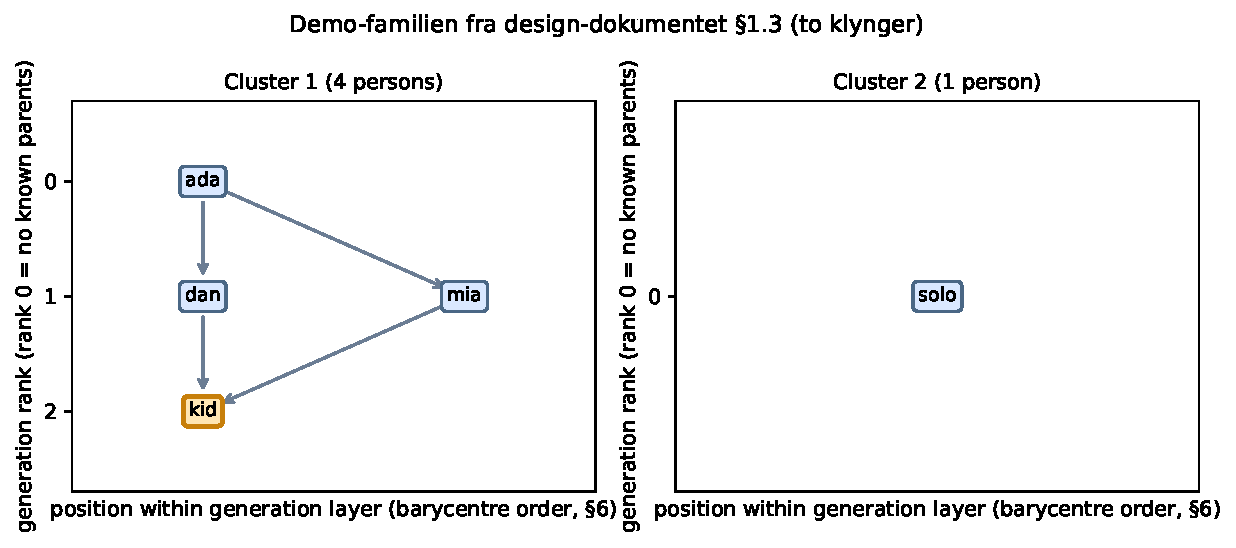
\includegraphics[width=0.95\textwidth]{figurer/familie_demo.pdf}
\caption{Demo-familien fra design-dokumentet \S 1.3 tegnet af programmets eget
view-modul. To klynger: sammenbrudsfamilien til venstre (ada er forælder til både
mia og dan, hvilket er pedigree-collapse, invariant \textbf{I3}) og den isolerede
person \texttt{solo} til højre. Søgeudgangspunktet \texttt{kid} er fremhævet.}
\end{figure}

\begin{figure}[h]
\centering
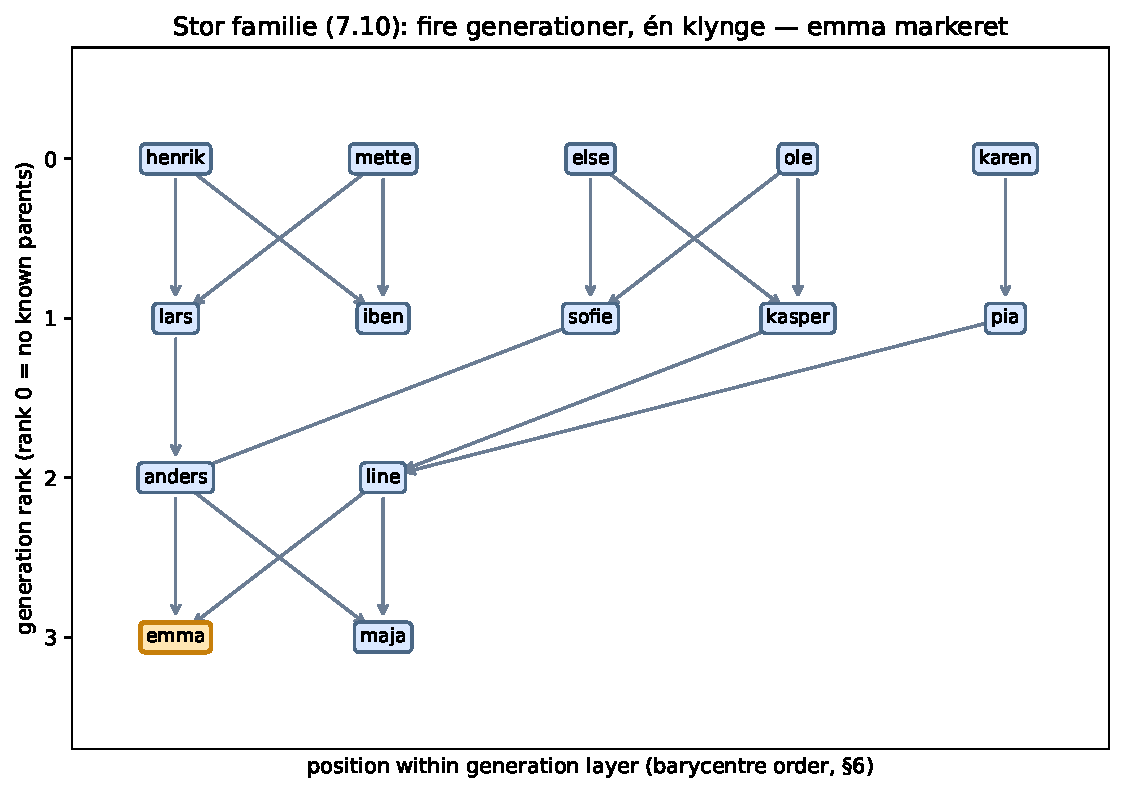
\includegraphics[width=0.8\textwidth]{figurer/stor_familie.pdf}
\caption{Den ``store familie'' fra opgave 7.10: 14 personer, fire generationer,
én klynge. Anders' mor \texttt{sofie} og lines far \texttt{kasper} er søskende,
så deres børn \texttt{emma} og \texttt{maja} har et sammenbrudt stamtræ på
\texttt{ole}/\texttt{else} --- programmets eget slægtskabsspørgsmål finder
præcis de to som fælles aner for \texttt{anders} og \texttt{line}.
\texttt{emma} er fremhævet.}
\end{figure}

\begin{figure}[h]
\centering
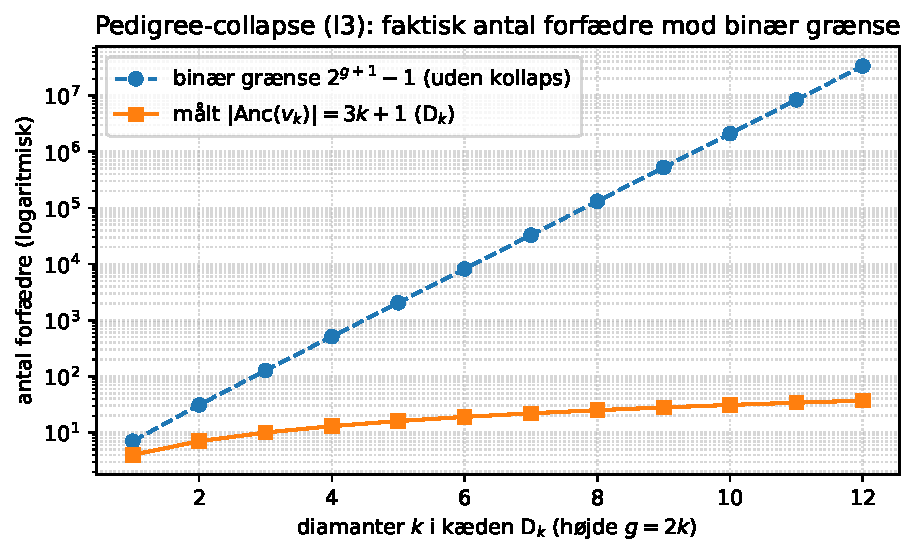
\includegraphics[width=0.8\textwidth]{figurer/pedigree_collapse.pdf}
\caption{Pedigree-collapse i tal: for diamantkæden $D_k$ er det faktiske antal
forfædre $|\mathrm{Anc}(v_k)| = 3k+1$, mens den naive bin{\ae}re gr{\ae}nse
$2^{g+1}-1$ vokser eksponentielt med h{\o}jden $g = 2k$. M{\aa}lt med programmets
\texttt{ancestors\_iterative}.}
\end{figure}

\begin{figure}[h]
\centering
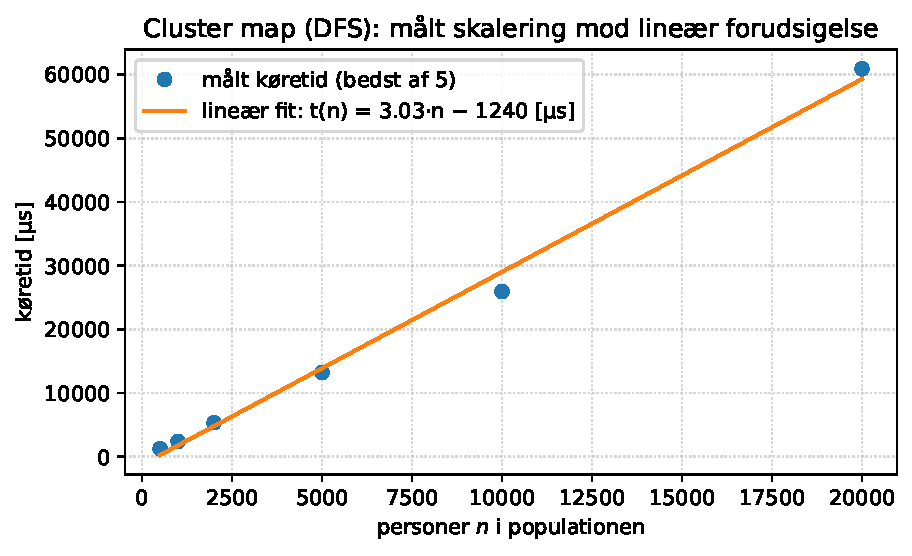
\includegraphics[width=0.8\textwidth]{figurer/scaling.pdf}
\caption{M{\aa}lt k{\o}retid for klusterkort-konstruktionen (DFS) vha.
\texttt{time.perf\_counter}, bedst af 5 gentagelser pr. punkt. Den line{\ae}re
fit $t(n) \approx c \cdot n$ bekr{\ae}fter kompleksitetsanalysen
$T = \Theta(n + m) = \Theta(n)$ fra \S 4.1 (invariant \textbf{I1} giver
$m \le 2n$).}
\end{figure}

% ═════════════════════════════════════════════════════════════════════════════
\section*{Bilag D. Udviklingsprocessen (Git)}
% ═════════════════════════════════════════════════════════════════════════════

Koden er udviklet på \texttt{dev}-branchen i repoet
\begin{center}
\url{https://github.com/ExperiencesXP/proj_herritage_tree}
\end{center}
Commit-oversigten pr. 2026-10-07 (nyeste øverst; den afsluttende commit til
bilagene ligger øverst i repoet):

\begin{center}\footnotesize
\begin{tabular}{@{}llp{6,9cm}@{}}
\toprule
\textbf{Hash} & \textbf{Dato} & \textbf{Besked} \\
\midrule
\texttt{8c218d7} & 2026-10-07 22:31 & feat: implement 7.10 kinship queries (\texttt{find\_common\_ancestor}, \texttt{is\_related}) \\
\texttt{d3aad43} & 2026-10-07 20:00 & docs: add synopsis material (figures, LaTeX appendix, writing notes) \\
\texttt{c163937} & 2026-10-07 19:49 & docs: fix clone URL and document running, tests and MVC layers \\
\texttt{c35db37} & 2026-10-07 19:49 & feat: add matplotlib visualization and MVC controller \\
\texttt{893432f} & 2026-10-07 19:49 & fix: use visited-guarded goal search over the undirected shadow \\
\texttt{094749d} & 2026-10-07 19:44 & fix: repair \texttt{\_\_str\_\_} parent-slot text and pairs-map arrow orientation \\
\texttt{f7fc0e7} & 2026-10-05 13:45 & works on my machine bro \\
\texttt{8dd1ba4} & 2026-10-01 11:56 & Wire the finalized entry point: \texttt{poetry run python src} \\
\texttt{47d965a} & 2026-10-01 11:27 & Implement cluster map and recursive search per design doc \\
\texttt{20e2447} & 2026-10-01 10:02 & do this and that \\
\texttt{f724764} & 2026-09-29 21:45 & becoming woke \\
\texttt{a8c0032} & 2026-09-28 15:16 & Initial commit \\
\bottomrule
\end{tabular}
\end{center}

\bigskip
\noindent\fbox{\parbox{0.95\textwidth}{\centering
SKÆRMDUMP 1 (indsat her): Git Graph i VS Code (udvidelsen \emph{Git Graph}) med
grenen \texttt{dev} og alle commits.}}

\bigskip
\noindent\fbox{\parbox{0.95\textwidth}{\centering
SKÆRMDUMP 2 (indsat her): commit-oversigt med datoer ---
\url{https://github.com/ExperiencesXP/proj_herritage_tree/commits/dev}.}}

% ═════════════════════════════════════════════════════════════════════════════
\section*{Bilag E. Verifikation: kørsel og tests}
% ═════════════════════════════════════════════════════════════════════════════

\texttt{poetry run pytest} giver 25 tests, som dækker verifikationsplanens \S 8:
klusterkort sammenlignes med en uafhængig BFS-reference, identitet (3)
$k = n - s$ holdes på tilfældige populationer, dybe kæder klarer de iterative
traverseringer, cyklusser afvises, skaleringen er nær-lineær,
slægtskabsspørgsmålet fra \S 7.10 er dækket (\texttt{find\_common\_ancestor},
\texttt{is\_related}), og \texttt{Person}-klassens opførsel er fastholdt
(\texttt{\_\_str\_\_}, standardnavne efter stedord).

Udskrift fra \texttt{poetry run python src} (uddrag):

\begin{lstlisting}[basicstyle=\ttfamily\footnotesize]
Heritage-tree cluster map (docs/cluster_map_and_recursive_search.md)
population  n = 5, parent edges m = 4  (I1: m <= 2n)
clusters    k = 2  (identity 3: k = n - s with s = 3)
  C2: 1 persons - solo
  C1: 4 persons - ada, dan, kid, mia
cluster of kid (explore_iterative over G-bar): ada, dan, kid, mia
ancestors of kid: 4 - ada, dan, kid, mia  (pedigree collapse reduces
the binary-lattice bound)
descendants of ada: 3 - dan, kid, mia
early-exit search found: ada (O7)
common ancestors of mia and dan: ada
is_related(mia, dan) = True
is_related(kid, solo) = False

layered layout (ranks and crossing counts):
  C1: ranks [0, 1, 2], crossings = 1
  C2: ranks [0], crossings = 0
\end{lstlisting}

Bem{\ae}rk identiteten i praksis: $n = 5$, $m = 4$ forældreferencer,
$s = 3$ vellykkede sammenl{\aa}gninger, $k = 2$ klynger --- og
$k = n - s = 5 - 3 = 2$.

% ═════════════════════════════════════════════════════════════════════════════
\section*{Bilag F. Kravdokumentation: produktet vs. kravene}
% ═════════════════════════════════════════════════════════════════════════════

Kravene stammer fra Projekt.docx (produkt, visualisering, MVC) og afsnit 7.10 i
bogen (\emph{Projekt: Fælles aner}, s. 162--163). Koden er bevidst skrevet på
engelsk; attributterne \texttt{name}, \texttt{mom}, \texttt{dad} svarer til
diagrammets \texttt{navn}, \texttt{mor}, \texttt{far}.

\begin{center}\footnotesize
\begin{tabular}{@{}p{6,4cm}p{8,4cm}@{}}
\toprule
\textbf{Krav} & \textbf{Opfyldt af} \\
\midrule
Program der kan undersøge slægtskab (``Har to personer mindst en fælles ane?'')
  & \texttt{search.is\_related()} og \texttt{find\_common\_ancestor()} (B8) \\
Person med valgfri mor og far
  & \texttt{Person(name, mom, dad)} (B1) \\
Klassediagrammets attributter
  & \texttt{name}/\texttt{mom}/\texttt{dad} (engelsk) + \texttt{pronouns} \\
Opret personer og forbind dem
  & \texttt{build\_family\_graph} (B2) \\
\texttt{\_\_str\_\_} a la ``Navn Nikolaj, mors navn er Anne...''
  & \texttt{Person.\_\_str\_\_} (B1) \\
Test af \texttt{\_\_str\_\_}
  & \texttt{test\_person\_dunder\_str\_matches\_book\_style} \\
Standardnavne efter stedord (John/Jane/Alex Doe)
  & \texttt{test\_default\_name\_follows\_pronouns} \\
Stor familie, mindst tre generationer
  & figur \texttt{stor\_familie.pdf} (14 personer, 4 generationer) \\
Tegn et stamtræ
  & \texttt{view.render\_cluster} (B7) \\
\texttt{find\_common\_ancestor()} returnerer liste over fælles aner
  & \texttt{search.find\_common\_ancestor()} (B8) \\
\texttt{is\_related()} returnerer boolean
  & \texttt{search.is\_related()} (B8) \\
Visualisering med \texttt{matplotlib.pyplot}
  & \texttt{src/view.py} (B7) \\
MVC-arkitektur
  & bilag A: model / controller / view \\
\bottomrule
\end{tabular}
\end{center}

\bigskip
\noindent\textbf{Svar på spørgsmålet ``Hvilken type relation er der tale om?''}
Forbindelsen mellem \texttt{Person}-objekterne er en \emph{assosiation} ---
mere præcist \emph{aggregering} (``har en''-relation): et objekt har referencer
til andre \texttt{Person}-objekter som mor/far, objekterne eksisterer uafhængigt
af hinanden, relationen er valgfri (\texttt{None}), og den er \emph{refleksiv}
--- samme klasse i begge ender. Det er ikke nedarvning.

\bigskip
\noindent\textbf{Definition-valg.} Spørgsmålet er om \emph{mindst} en fælles
ane. $\mathrm{Anc}(v)$ indeholder per \S 2.5 også personen selv, så en forælder
og et barn tælles som beslægtede --- ellers ville \texttt{is\_related(ada, kid)}
give \texttt{False}, uagtet at ada er kids bedstemor.

\end{document}
